% !TEX program = xelatex
\documentclass[10pt, aspectratio=169]{beamer}

\usepackage{fontspec}
\usepackage{polyglossia}
\setdefaultlanguage{vietnamese}
\setotherlanguage{english}
\setmainfont{Times New Roman}
\setsansfont{Calibri}

\usepackage{graphicx}
\usepackage{booktabs}
\usepackage{tabularx}
\usepackage{colortbl}
\usepackage{tikz}
\usepackage{multicol}
\usepackage{caption}
\usepackage{multirow}
\usepackage{array}
\usepackage{amsmath}
\usepackage{amssymb}
\usepackage{xcolor}
\usepackage{appendixnumberbeamer}

% =====================  Theme USTH Blue  =====================
\definecolor{usthblue}{RGB}{0, 84, 166}
\definecolor{usthlight}{RGB}{220, 232, 247}
\definecolor{usthred}{RGB}{237, 28, 36}
\definecolor{usthaccent}{RGB}{0, 132, 209}
\definecolor{usthdark}{RGB}{0, 51, 102}
\definecolor{softgray}{RGB}{245, 245, 245}
\definecolor{goodgreen}{RGB}{34, 139, 34}

\usetheme{Madrid}
\usecolortheme[named=usthblue]{structure}
\setbeamercolor{title}{fg=white,bg=usthblue}
\setbeamercolor{frametitle}{fg=white,bg=usthblue}
\setbeamercolor{block title}{fg=white,bg=usthaccent}
\setbeamercolor{block body}{bg=usthlight!40}
\setbeamercolor{item}{fg=usthblue}
\setbeamercolor{section in toc}{fg=usthdark}
\setbeamertemplate{navigation symbols}{}
\setbeamertemplate{blocks}[rounded][shadow=true]
\setbeamertemplate{itemize item}{\color{usthblue}$\blacktriangleright$}
\setbeamertemplate{itemize subitem}{\color{usthaccent}$\bullet$}

% Footer gọn
\setbeamertemplate{footline}{%
  \leavevmode%
  \hbox{%
    \begin{beamercolorbox}[wd=.32\paperwidth,ht=2.4ex,dp=1ex,left]{author in head/foot}%
      \hspace*{2ex}\insertshortauthor
    \end{beamercolorbox}%
    \begin{beamercolorbox}[wd=.45\paperwidth,ht=2.4ex,dp=1ex,center]{title in head/foot}%
      \insertshorttitle
    \end{beamercolorbox}%
    \begin{beamercolorbox}[wd=.23\paperwidth,ht=2.4ex,dp=1ex,right]{date in head/foot}%
      \insertframenumber{} / \inserttotalframenumber\hspace*{2ex}
    \end{beamercolorbox}}%
}

% =====================  Thông tin  =====================
\title[Phân loại Tổn thương Da bằng Học sâu]{\large Đánh giá So sánh các Mô hình Học sâu \\ cho Bài toán Phân loại Tổn thương Da trên Ảnh Dermoscopy}
\subtitle{\small Tiếp cận Ensemble và Khả diễn giải bằng Grad-CAM}
\author[Nguyễn Trọng Bách]{Nguyễn Trọng Bách \textemdash{} 23BI14057 \\[2pt]
\footnotesize \textbf{GVHD nội bộ:} TS. Nghiêm Thị Phương \quad \textbf{GVHD bên ngoài:} TS. Vũ Trọng Sinh}
\institute[USTH]{\footnotesize Khoa Công nghệ Thông tin và Truyền thông \\ Đại học Khoa học và Công nghệ Hà Nội}
\date{\footnotesize Tháng 7, 2026}

\titlegraphic{
\includegraphics[height=1.3cm]{../thesis/figures/logo.png}}

\begin{document}

% =====================  Trang bìa  =====================
\begin{frame}[plain]
    \titlepage
\end{frame}

% =====================  Mục lục  =====================
\begin{frame}{Nội dung trình bày}
    \begin{columns}
        \column{0.55\textwidth}
        \tableofcontents[hideallsubsections]
        \column{0.45\textwidth}
        \begin{block}{Trọng tâm khóa luận}
            \footnotesize
            Xây dựng và đánh giá một pipeline học sâu hoàn chỉnh cho phân loại 7 lớp tổn thương da trên ISIC 2018,\,kết hợp \textbf{4 kiến trúc} bằng \textbf{soft-voting ensemble} và diễn giải kết quả bằng \textbf{Grad-CAM}.
        \end{block}
    \end{columns}
\end{frame}

% =========================================================
\section{Giới thiệu}
% =========================================================
\begin{frame}{Bối cảnh và động lực}
    \begin{columns}[T]
        \column{0.55\textwidth}
        \begin{block}{Vấn đề lâm sàng}
            \footnotesize
            Ung thư hắc tố chiếm phần lớn số tử vong do ung thư da, nhưng tỷ lệ sống sau 5 năm vượt \textbf{99\%} nếu phát hiện sớm. Dermoscopy giúp quan sát tổn thương ở mức không xâm lấn, song việc diễn giải phụ thuộc nặng vào kinh nghiệm bác sĩ.
        \end{block}
        \vspace{0.2cm}
        \textbf{Ba trở ngại của AI hỗ trợ chẩn đoán:}
        \begin{itemize}\footnotesize
            \item \textbf{Mất cân bằng dữ liệu} — lớp đa số áp đảo các lớp ác tính hiếm.
            \item \textbf{Tương đồng hình thái} — Melanoma và Nevus dễ nhầm lẫn.
            \item \textbf{Hộp đen} — bác sĩ khó tin cậy nếu không có giải thích.
        \end{itemize}

        \column{0.45\textwidth}
        \begin{figure}
            \centering
            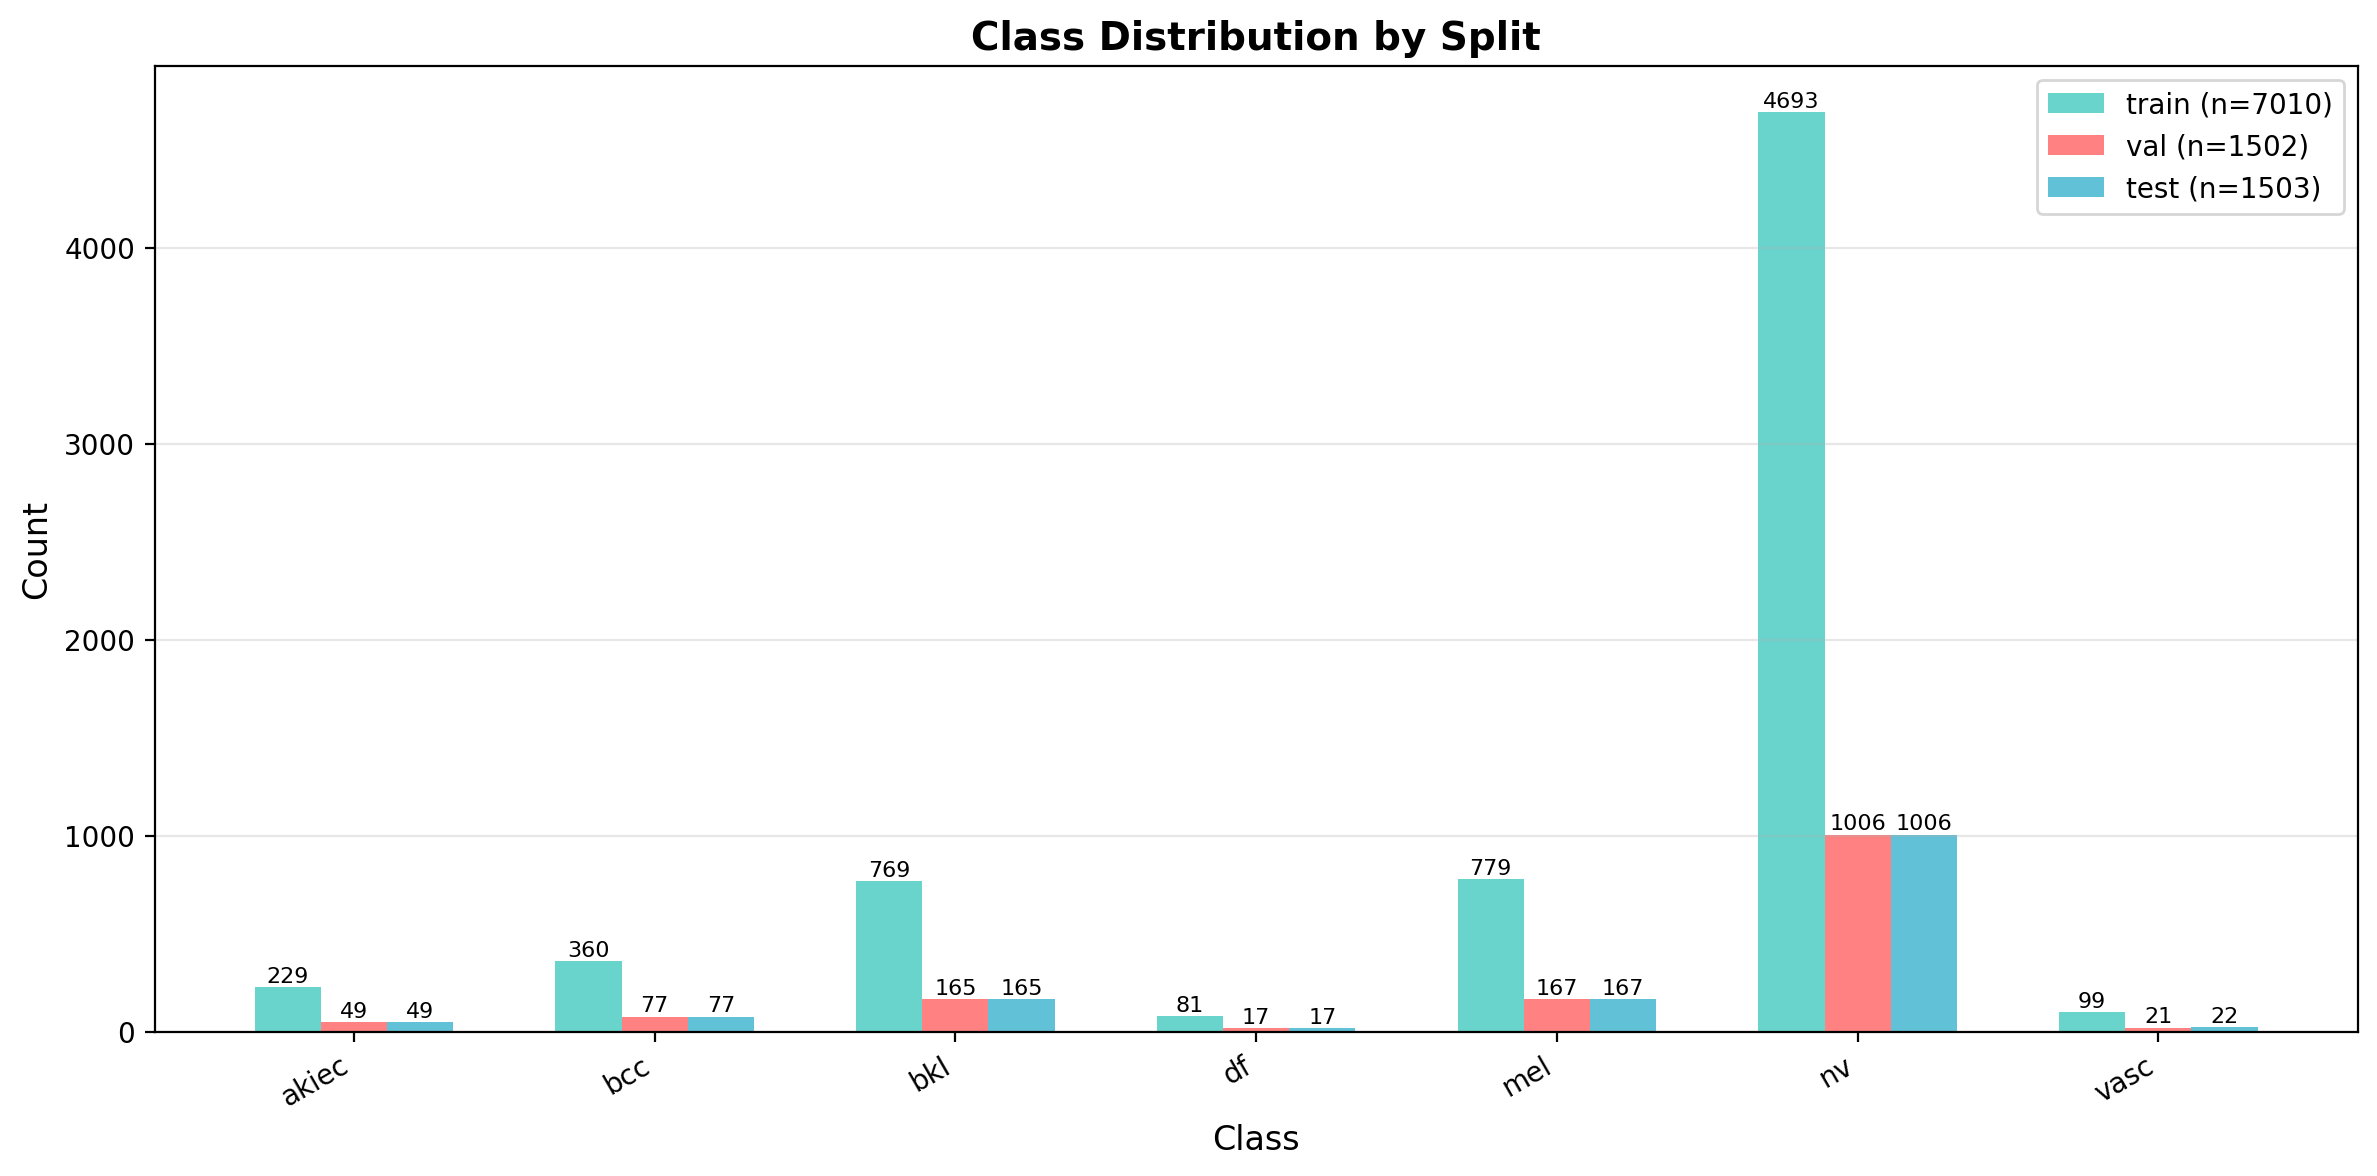
\includegraphics[width=\linewidth,height=5cm,keepaspectratio]{../thesis/figures/class_distribution.png}
            \captionsetup{font=scriptsize}
            \caption{Phân bố 7 lớp trong ISIC 2018 — tỉ lệ NV:DF lên tới 58:1.}
        \end{figure}
    \end{columns}
\end{frame}

\begin{frame}{Mục tiêu khóa luận}
    \begin{columns}[T]
        \column{0.5\textwidth}
        \begin{block}{Mục tiêu chính}
            \footnotesize
            Xây dựng pipeline tự động phân loại \textbf{7 loại tổn thương da} từ ảnh dermoscopy, đạt độ chính xác cao đồng thời \textbf{khả diễn giải} cho mục đích lâm sàng.
        \end{block}

        \column{0.5\textwidth}
        \textbf{Bốn đóng góp cụ thể}
        \begin{enumerate}\footnotesize
            \item Pipeline xử lý mất cân bằng bằng Weighted Sampler, Mixup, CutMix, Label Smoothing.
            \item So sánh \textbf{4 kiến trúc} (CNN $+$ Transformer) trên cùng một pipeline.
            \item \textbf{Soft-voting ensemble} đẩy hiệu năng vượt mô hình đơn.
            \item \textbf{Grad-CAM} cùng prototype Streamlit để bác sĩ kiểm tra trực quan.
        \end{enumerate}
    \end{columns}

    \vspace{0.3cm}
    \begin{center}
    \footnotesize \textcolor{usthdark}{\textbf{Kim chỉ nam:} ưu tiên \textit{Macro F1} và \textit{Macro AUC} — không để Accuracy lừa.}
    \end{center}
\end{frame}

% =========================================================
\section{Dữ liệu và thách thức}
% =========================================================
\begin{frame}{Bộ dữ liệu ISIC 2018 Task 3}
    \begin{columns}[T]
        \column{0.46\textwidth}
        \footnotesize
        \textbf{HAM10000 — chuẩn benchmark dermoscopy:}
        \begin{itemize}
            \item \textbf{10.015} ảnh, \textbf{7} lớp tổn thương.
            \item Chia theo \textit{stratified sampling} 70/15/15.
            \item Mỗi split giữ nguyên tỉ lệ 7 lớp.
        \end{itemize}

        \vspace{0.2cm}
        \begin{block}{Chỉ số ưu tiên}
            \footnotesize Vì lớp NV chiếm 67\% nên Accuracy không phản ánh đúng. Ta đo bằng \textbf{Macro F1} và \textbf{Macro AUC} — bình đẳng với mọi lớp.
        \end{block}

        \column{0.54\textwidth}
        \scriptsize
        \begin{table}[]
            \centering
            \begin{tabular}{lrrrrr}
            \toprule
            \rowcolor{usthblue!25} \textbf{Lớp} & \textbf{Train} & \textbf{Val} & \textbf{Test} & \textbf{Tổng} & \textbf{\%} \\
            \midrule
            NV (Nevus)          & 4\,693 & 1\,006 & 1\,006 & \textbf{6\,705} & 66.9 \\
            MEL (Melanoma)      &   779  &  167   &  167   & 1\,113 & 11.1 \\
            BKL (Benign Ker.)   &   769  &  165   &  165   & 1\,099 & 11.0 \\
            BCC (Basal Cell)    &   360  &   77   &   77   &   514  &  5.1 \\
            AKIEC (Actinic)     &   229  &   49   &   49   &   327  &  3.3 \\
            VASC (Vascular)     &    99  &   21   &   22   &   142  &  1.4 \\
            DF (Dermatofibroma) &    81  &   17   &   17   &   115  &  1.1 \\
            \midrule
            \textbf{Tổng}       & \textbf{7\,010} & \textbf{1\,502} & \textbf{1\,503} & \textbf{10\,015} & 100 \\
            \bottomrule
            \end{tabular}
        \end{table}

        \vspace{0.15cm}
        \centering
        \textcolor{usthred}{\footnotesize Tỉ lệ mất cân bằng cực đoan: \textbf{NV : DF $\approx$ 58 : 1}}
    \end{columns}
\end{frame}

\begin{frame}{Hệ quả của mất cân bằng dữ liệu}
    \begin{columns}[T]
        \column{0.55\textwidth}
        \footnotesize
        \textbf{Tại sao mất cân bằng là vấn đề nghiêm trọng?}
        \begin{itemize}
            \item Mạng nơ-ron tối thiểu hóa loss tổng thể $\Rightarrow$ ưu tiên lớp đa số.
            \item Dự đoán "NV cho mọi ảnh" vẫn cho $\sim$67\% Accuracy --- nhưng vô dụng lâm sàng.
            \item Lớp DF, VASC, AKIEC có $<$\,250 ảnh huấn luyện --- rất dễ \textit{memorize} thay vì học features.
        \end{itemize}

        \vspace{0.2cm}
        \begin{block}{Bốn cơ chế đối phó trong pipeline}
            \footnotesize
            \begin{enumerate}
                \item \textbf{Weighted Random Sampler} cân bằng mini-batch.
                \item \textbf{Mixup / CutMix} làm mịn ranh giới quyết định.
                \item \textbf{Label Smoothing} chống over-confidence.
                \item \textbf{Macro F1} làm tiêu chí chọn checkpoint.
            \end{enumerate}
        \end{block}

        \column{0.45\textwidth}
        \begin{figure}
            \centering
            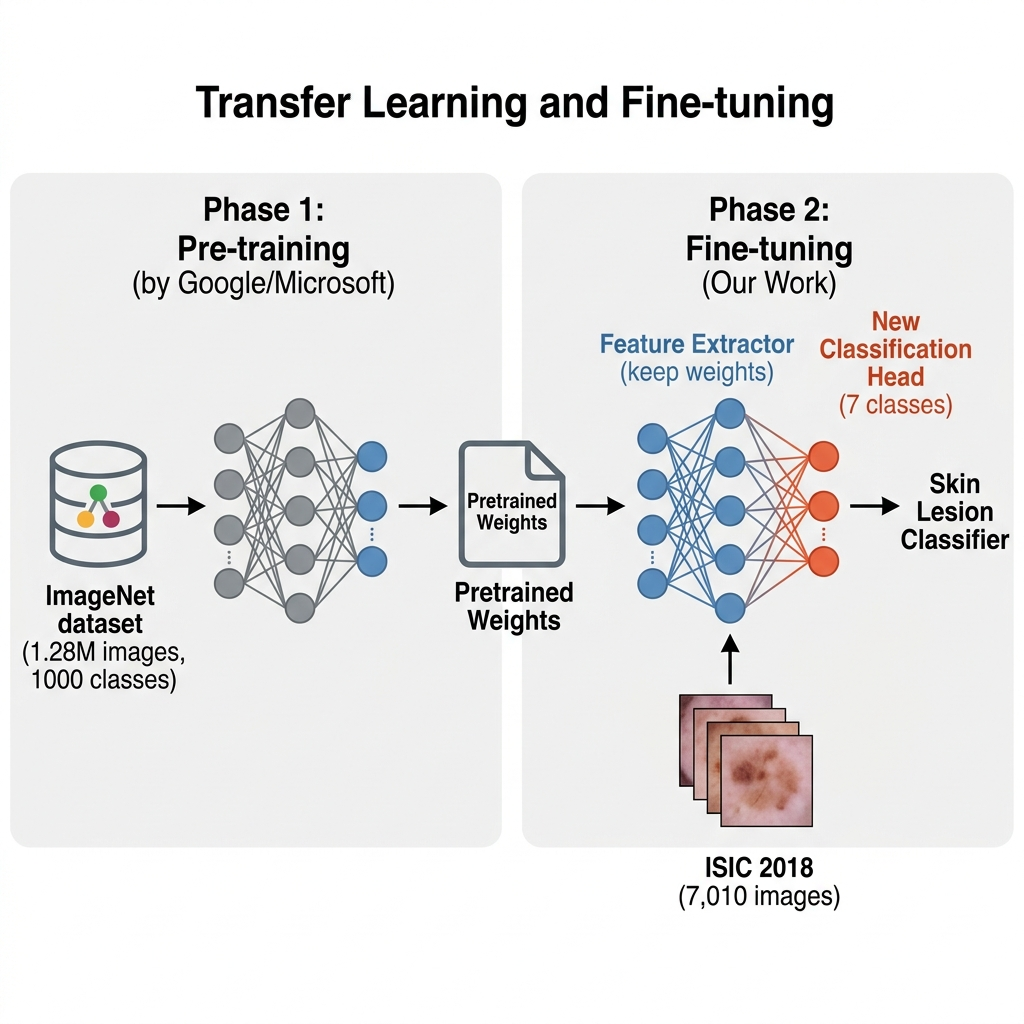
\includegraphics[width=\linewidth,height=5cm,keepaspectratio]{../thesis/figures/transfer_learning.png}
            \captionsetup{font=scriptsize}
            \caption{Transfer learning từ ImageNet sang ISIC: tái sử dụng features tổng quát, chỉ thay classifier head.}
        \end{figure}
    \end{columns}
\end{frame}

% =========================================================
\section{Phương pháp}
% =========================================================
\begin{frame}{Pipeline tổng quan}
    \begin{figure}
        \centering
        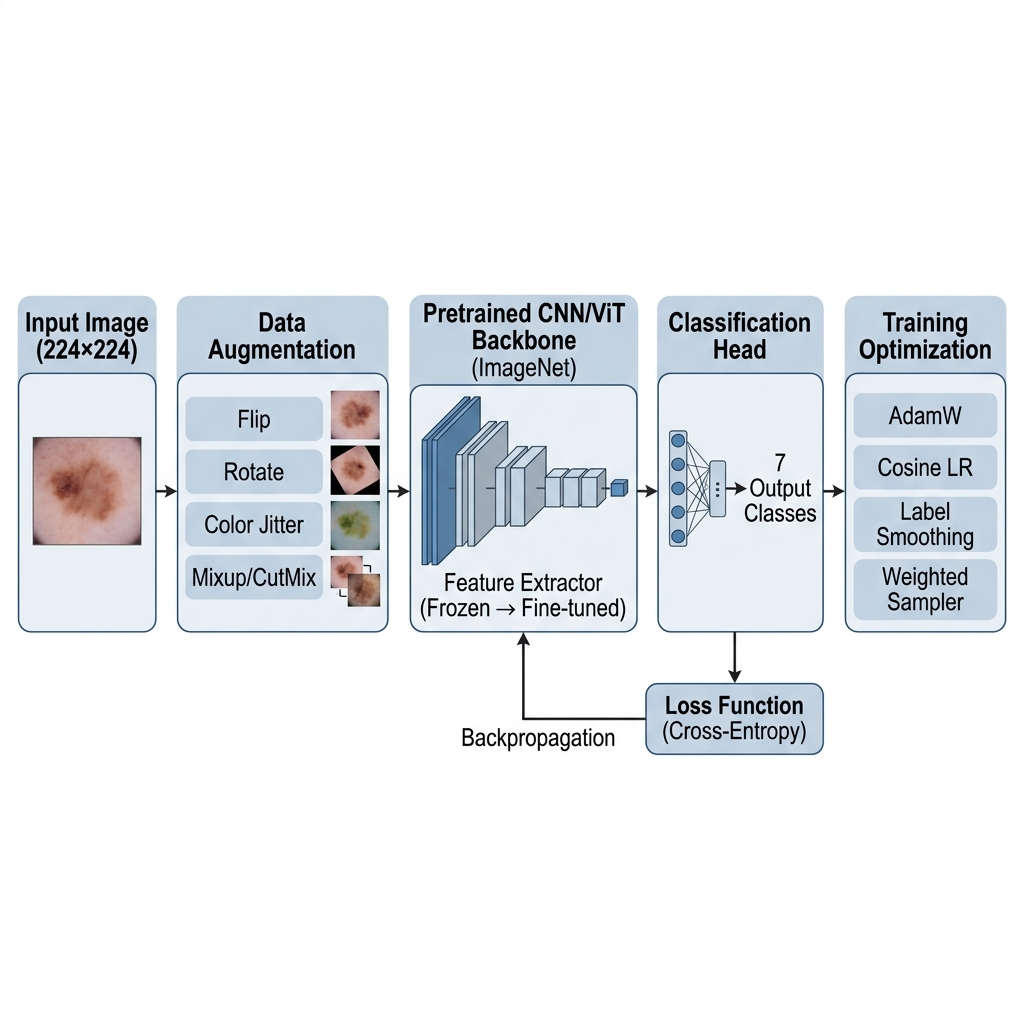
\includegraphics[height=0.72\textheight,keepaspectratio]{../thesis/figures/training_pipeline.png}
        \captionsetup{font=scriptsize}
        \caption{Sơ đồ pipeline: tiền xử lý ảnh, augmentation, weighted sampler, Mixup/CutMix, fine-tune mô hình pretrained, đánh giá trên test set.}
    \end{figure}
\end{frame}

\begin{frame}{Bốn kiến trúc được so sánh}
    \scriptsize
    \begin{table}[]
        \centering
        \begin{tabular}{lcll}
        \toprule
        \rowcolor{usthblue!25}
        \textbf{Mô hình} & \textbf{Tham số} & \textbf{Nguyên tắc thiết kế} & \textbf{Vai trò trong ensemble} \\
        \midrule
        EfficientNet-B0 & 5.3M  & MBConv $+$ SE, compound scaling           & CNN gọn, đặc trưng local mịn  \\
        ResNet50        & 25.6M & Bottleneck residual                       & CNN sâu, baseline cổ điển     \\
        DenseNet121     & 8.0M  & Dense connectivity, tái sử dụng features  & CNN tận dụng feature reuse    \\
        Swin-Tiny       & 28.0M & Shifted-window self-attention             & Vision Transformer, ngữ cảnh toàn cục \\
        \bottomrule
        \end{tabular}
    \end{table}

    \vspace{0.3cm}
    \footnotesize
    \begin{itemize}
        \item Tất cả mô hình \textbf{fine-tune từ ImageNet pretrained} qua thư viện \texttt{timm}.
        \item Đầu ra thay bằng \texttt{Linear($d$, 7)}, dropout 0.25--0.30 trước classifier.
        \item Lựa chọn 4 kiến trúc đa dạng để ensemble khai thác \textbf{lỗi không tương quan} giữa CNN và Transformer.
    \end{itemize}
\end{frame}

\begin{frame}{Chiến lược huấn luyện}
    \begin{columns}[T]
        \column{0.5\textwidth}
        \begin{block}{Mixup \& CutMix\ \footnotesize($p = 0.5$ mỗi loại)}
            \scriptsize
            \textbf{Mixup:} $\tilde{x} = \lambda x_i + (1-\lambda) x_j$ với $\lambda \sim \mathrm{Beta}(0.2, 0.2)$.\\[2pt]
            \textbf{CutMix:} dán patch ngẫu nhiên giữa hai ảnh, nhãn lai theo tỉ lệ diện tích.\\[3pt]
            $\Rightarrow$ ngăn memorize sample hiếm, làm mịn ranh giới quyết định.
        \end{block}

        \begin{block}{Label Smoothing\ \footnotesize($\varepsilon = 0.1$)}
            \scriptsize
            $y_{\text{smooth}} = (1-\varepsilon) \cdot y_{\text{onehot}} + \varepsilon / C$\\[2pt]
            $\Rightarrow$ giảm over-confidence, cải thiện calibration.
        \end{block}

        \column{0.5\textwidth}
        \begin{block}{Weighted Random Sampler}
            \scriptsize
            Trọng số mỗi mẫu: $w_c = \dfrac{N}{C \cdot n_c}$\\[2pt]
            Mỗi batch xấp xỉ cân bằng 7 lớp \textemdash{} tăng exposure cho DF/VASC.
        \end{block}

        \begin{block}{Cấu hình tối ưu}
            \scriptsize
            \textbf{Optimizer:} AdamW, cosine annealing $+$ linear warmup.\\
            \textbf{Mixed precision:} FP16 (giảm $\sim$40\% bộ nhớ GPU).\\
            \textbf{Gradient clipping:} $\|\nabla\|_{\max} = 1.0$.\\
            \textbf{Early stopping:} patience $= 12$ epoch theo Macro F1.
        \end{block}
    \end{columns}
\end{frame}

\begin{frame}{Siêu tham số theo mô hình}
    \scriptsize
    \begin{table}[]
        \centering
        \begin{tabular}{lcccc}
        \toprule
        \rowcolor{usthblue!25}
        \textbf{Hyperparameter} & \textbf{EfficientNet-B0} & \textbf{ResNet50} & \textbf{DenseNet121} & \textbf{Swin-Tiny} \\
        \midrule
        Learning rate       & 3e-4  & 3e-4 & 2.5e-4 & \textbf{1e-4} \\
        Weight decay        & 1e-3  & 1e-3 & 1e-3   & \textbf{5e-2} \\
        Warmup epochs       & 3     & 3    & 3      & 5 \\
        Max epochs          & 50    & 50   & 50     & 50 \\
        Batch size          & 16    & 16   & 16     & 16 \\
        Dropout             & 0.30  & 0.30 & 0.25   & 0.30 \\
        Mixup / CutMix $\alpha$ & 0.2 / 1.0 & 0.2 / 1.0 & 0.2 / 1.0 & 0.2 / 1.0 \\
        Label smoothing $\varepsilon$ & 0.1 & 0.1 & 0.1 & 0.1 \\
        \bottomrule
        \end{tabular}
    \end{table}

    \vspace{0.3cm}
    \begin{block}{Swin-Tiny tại sao khác biệt?}
        \footnotesize
        Transformer thiếu \textit{inductive bias} của CNN $\Rightarrow$ cần \textbf{learning rate thấp} (1e-4) để không phá vỡ attention weights pretrained, và \textbf{weight decay cao} (5e-2) để hạn chế overfit trên dataset nhỏ.
    \end{block}
\end{frame}

% =========================================================
\section{Kết quả thực nghiệm}
% =========================================================
\begin{frame}{Hiệu năng từng mô hình đơn}
    \scriptsize
    \begin{table}[]
        \centering
        \begin{tabular}{lcccccc}
        \toprule
        \rowcolor{usthblue!25}
        \textbf{Mô hình} & \textbf{Params} & \textbf{Epoch tốt nhất} & \textbf{Accuracy} & \textbf{Macro F1} & \textbf{AUC} & \textbf{Kappa} \\
        \midrule
        \textbf{EfficientNet-B0} & \textbf{5.3M} & 39 & \textbf{0.8836} & \textbf{0.8311} & 0.9522 & \textbf{0.7710} \\
        ResNet50                 & 25.6M & 39 & 0.8603 & 0.7902 & 0.9565 & 0.7309 \\
        DenseNet121              & 8.0M  & 49 & 0.8543 & 0.7967 & 0.9587 & 0.7206 \\
        Swin-Tiny                & 28.0M & \textbf{13} & 0.8490 & 0.7855 & \textbf{0.9600} & 0.7150 \\
        \bottomrule
        \end{tabular}
    \end{table}

    \vspace{0.3cm}
    \begin{columns}[T]
        \column{0.5\textwidth}
        \begin{block}{EfficientNet-B0 — quán quân đơn lẻ}
            \scriptsize
            Ít tham số nhất (5.3M) mà Accuracy và Macro F1 cao nhất. Compound scaling cộng với SE-blocks rất hợp với ảnh dermoscopy 224$\times$224.
        \end{block}

        \column{0.5\textwidth}
        \begin{block}{Swin-Tiny — paradox calibration}
            \scriptsize
            Overfit sớm nhất (epoch 13) nhưng AUC cao nhất 0.960. Cho thấy Swin xếp hạng xác suất tốt, nhưng quyết định cứng (argmax) thì kém hơn CNN.
        \end{block}
    \end{columns}
\end{frame}

\begin{frame}{Ensemble: kết hợp 4 mô hình bằng soft voting}
    \begin{columns}[T]
        \column{0.5\textwidth}
        \footnotesize
        \textbf{Cơ chế:} trung bình các vector xác suất đầu ra.
        \[
            \bar{p}(x) = \frac{1}{M}\sum_{m=1}^{M} p_m(x), \quad M = 4
        \]
        \begin{itemize}
            \item CNN bắt features cục bộ, Swin bắt ngữ cảnh toàn cục $\Rightarrow$ lỗi không tương quan.
            \item Trung bình xác suất \textbf{giảm phương sai dự đoán}.
            \item Không cần huấn luyện thêm, chỉ inference 4 lần.
        \end{itemize}

        \vspace{0.15cm}
        \begin{block}{Kết quả Ensemble (test set 1\,503 ảnh)}
            \centering \footnotesize
            Accuracy \textbf{89.49\%} \quad Macro F1 \textbf{0.845} \quad Macro AUC \textbf{0.980}
        \end{block}

        \column{0.5\textwidth}
        \begin{figure}
            \centering
            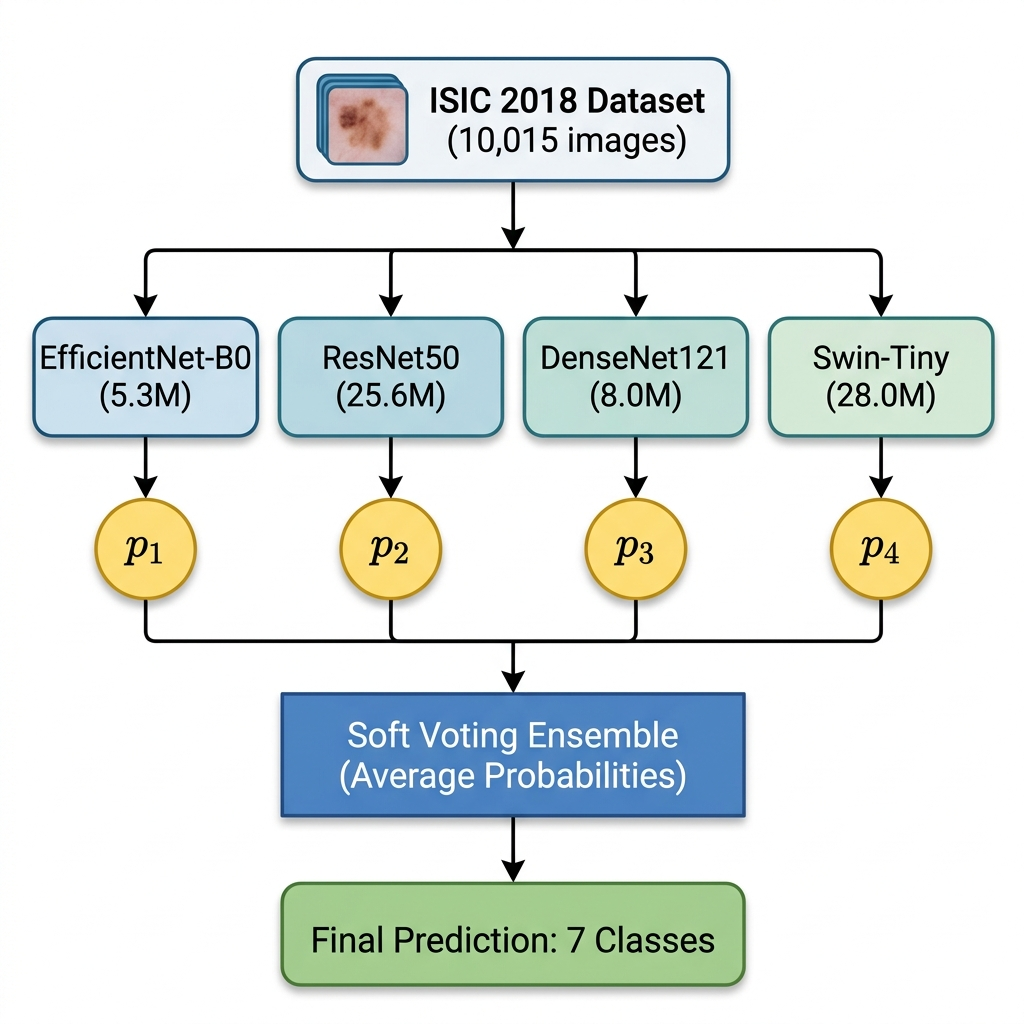
\includegraphics[width=\linewidth,height=5.5cm,keepaspectratio]{../thesis/figures/ensemble_architecture.png}
            \captionsetup{font=scriptsize}
            \caption{Kiến trúc soft-voting ensemble: 4 mô hình cùng inference, xác suất được trung bình trước khi argmax.}
        \end{figure}
    \end{columns}
\end{frame}

\begin{frame}{Phân tích chi tiết theo lớp (EB0 vs.\ Ensemble)}
    \scriptsize
    \begin{table}[]
        \centering
        \begin{tabular}{l|ccc|ccc}
        \toprule
        \rowcolor{usthblue!25} & \multicolumn{3}{c|}{\textbf{F1 theo lớp}} & \multicolumn{3}{c}{\textbf{AUC theo lớp}} \\
        \rowcolor{usthblue!25} \multirow{-2}{*}{\textbf{Lớp}} & \textbf{EB0} & \textbf{Ensemble} & \textbf{$\Delta$} & \textbf{EB0} & \textbf{Ensemble} & \textbf{$\Delta$} \\
        \midrule
        AKIEC & 0.717 & 0.710 & $-0.007$ & 0.921 & \textbf{0.972} & \textcolor{goodgreen}{$+0.051$} \\
        BCC   & 0.865 & 0.825 & $-0.040$ & 0.984 & \textbf{0.996} & $+0.012$ \\
        BKL   & 0.758 & \textbf{0.796} & \textcolor{goodgreen}{$+0.038$} & 0.938 & \textbf{0.968} & $+0.030$ \\
        DF    & 0.938 & 0.938 & $\phantom{-}0.000$ & 0.963 & \textbf{0.996} & $+0.033$ \\
        \rowcolor{usthlight} \textbf{MEL} & 0.695 & \textbf{0.744} & \textcolor{goodgreen}{\textbf{$+0.049$}} & 0.913 & \textbf{0.958} & \textcolor{goodgreen}{\textbf{$+0.045$}} \\
        NV    & 0.940 & \textbf{0.946} & $+0.006$ & 0.946 & \textbf{0.972} & $+0.026$ \\
        VASC  & 0.905 & \textbf{0.955} & \textcolor{goodgreen}{$+0.050$} & 1.000 & 1.000 & $\phantom{-}0.000$ \\
        \bottomrule
        \end{tabular}
    \end{table}

    \vspace{0.25cm}
    \begin{itemize}
        \footnotesize
        \item \textbf{Melanoma cải thiện rõ rệt} — lớp lâm sàng quan trọng nhất, F1 tăng $+4.9$\%, AUC tăng $+4.5$\%.
        \item \textbf{AUC tăng đồng đều} trên cả 7 lớp $\Rightarrow$ ensemble là công cụ \textit{xếp hạng rủi ro} mạnh.
        \item BCC giảm nhẹ F1 do Swin overconfident; bù lại AUC vẫn rất cao 0.996.
    \end{itemize}
\end{frame}

\begin{frame}{Ma trận nhầm lẫn của Ensemble}
    \begin{columns}[T]
        \column{0.42\textwidth}
        \footnotesize
        \textbf{Đọc ma trận:}
        \begin{itemize}
            \item Đường chéo cao $\Rightarrow$ recall tốt trên mọi lớp.
            \item \textbf{DF, VASC} hiếm nhưng vẫn được nhận diện chính xác --- nhờ Mixup $+$ Weighted Sampler.
            \item Nhầm lẫn còn lại tập trung ở cụm \textbf{MEL $\leftrightarrow$ NV $\leftrightarrow$ BKL}, vốn tương đồng hình thái.
            \item Không có lớp nào bị "biến mất" --- tránh được lỗi điển hình của mất cân bằng.
        \end{itemize}

        \column{0.58\textwidth}
        \begin{figure}
            \centering
            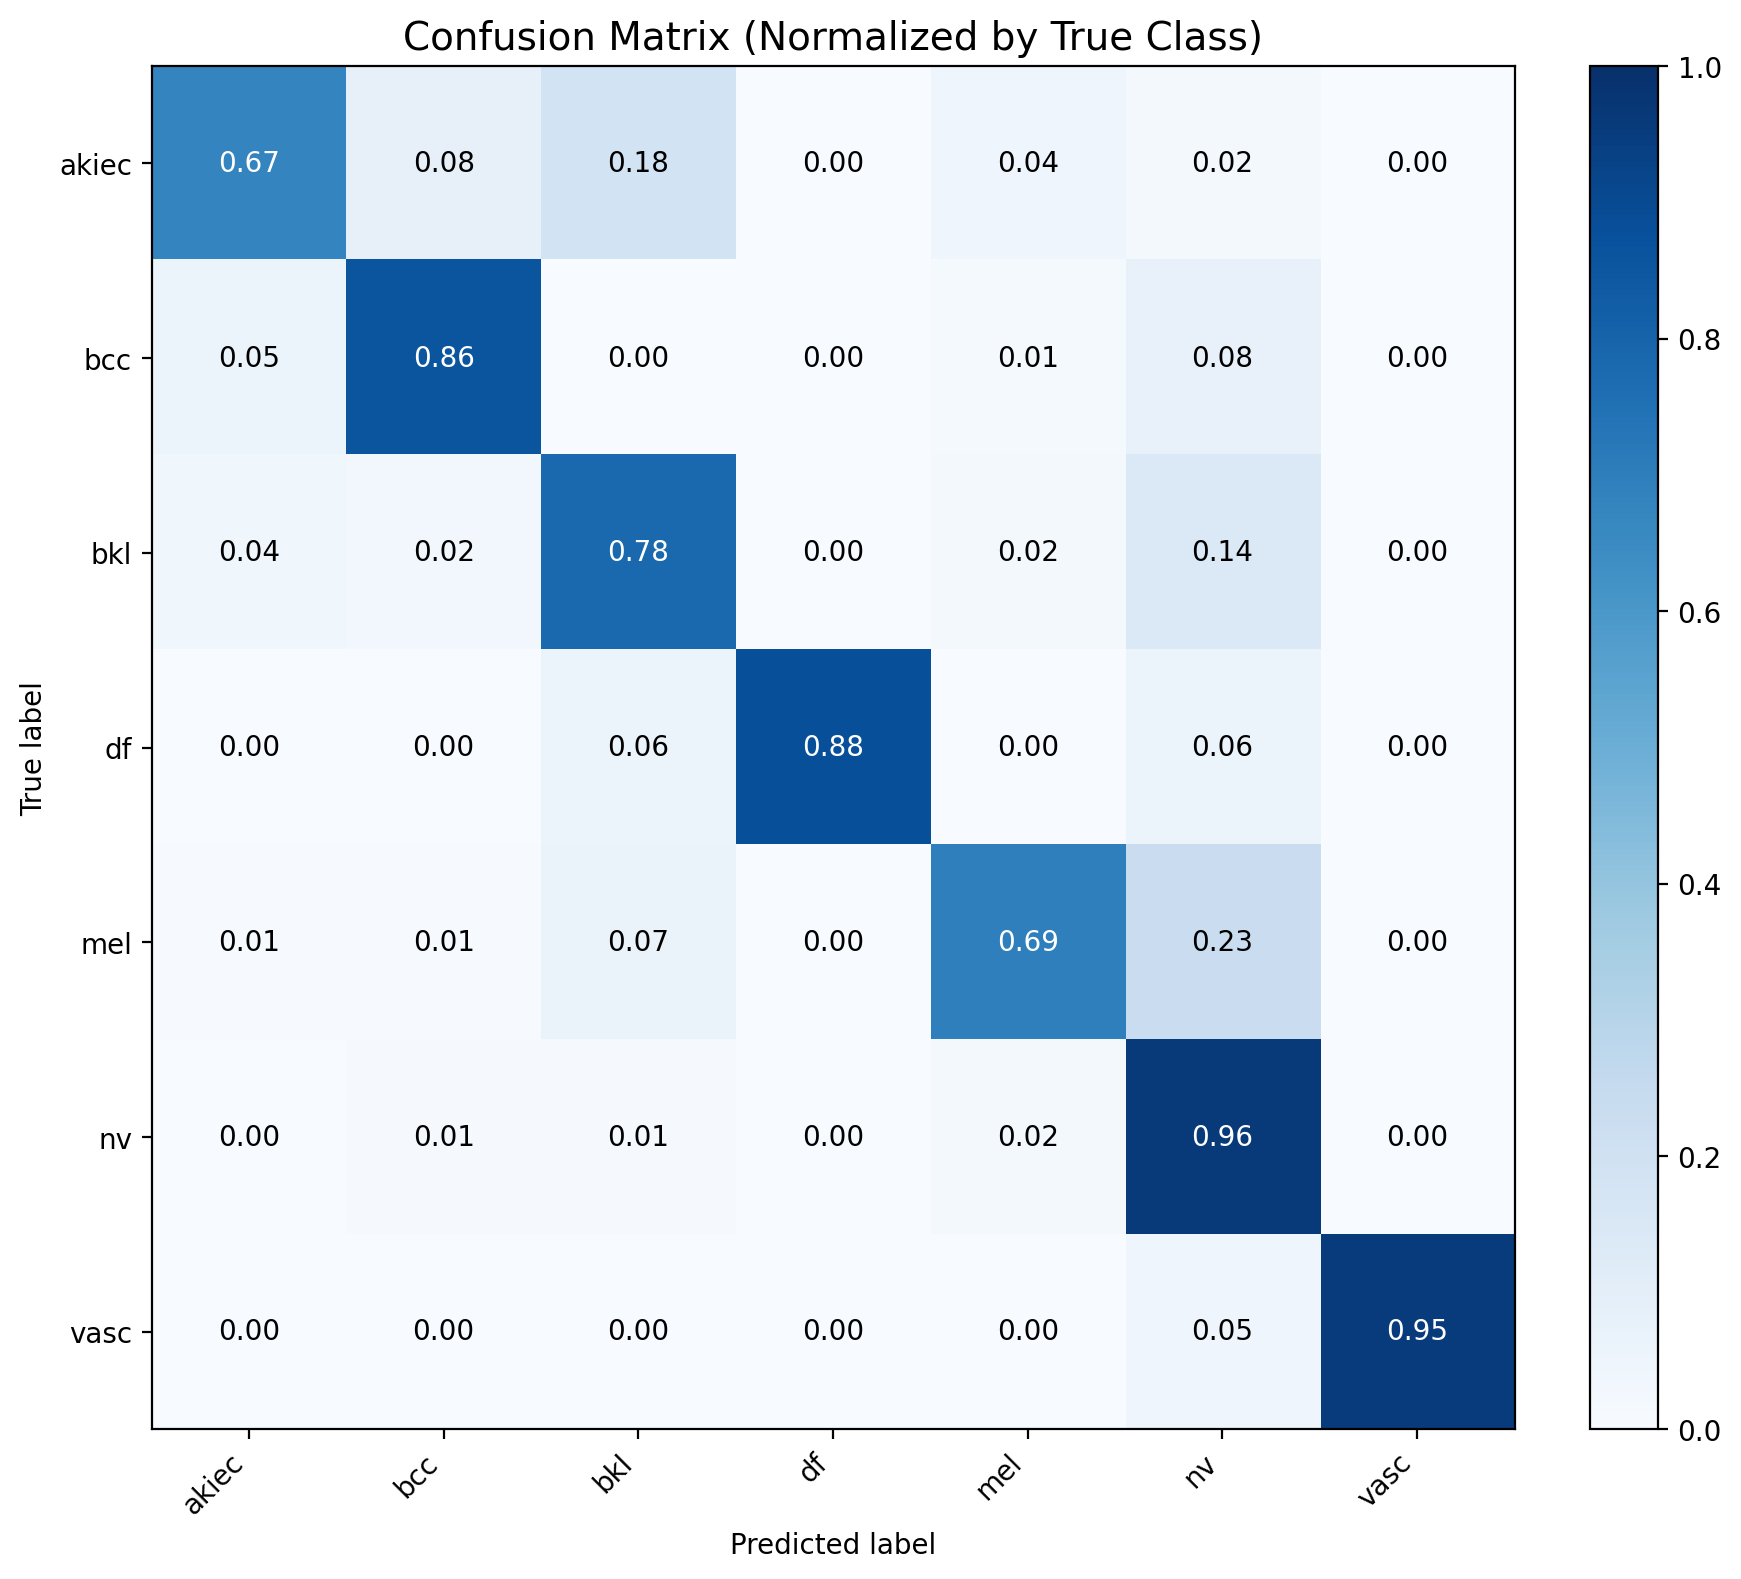
\includegraphics[height=6cm,keepaspectratio]{../thesis/figures/ensemble_confusion_matrix.png}
        \end{figure}
    \end{columns}
\end{frame}

% =========================================================
\section{Nghiên cứu loại bỏ thành phần}
% =========================================================
\begin{frame}{Ablation Study --- đóng góp của từng thành phần}
    \scriptsize
    \textit{Cùng EfficientNet-B0, lần lượt loại bỏ một thành phần để đo mức suy giảm Macro F1.}
    \vspace{0.2cm}
    \begin{table}[]
        \centering
        \begin{tabular}{lcccc}
        \toprule
        \rowcolor{usthblue!25}
        \textbf{Cấu hình} & \textbf{Accuracy} & \textbf{Macro F1} & \textbf{AUC} & \textbf{$\Delta$ Macro F1} \\
        \midrule
        \textbf{Full pipeline (baseline)} & \textbf{0.8836} & \textbf{0.8311} & 0.9522 & -- \\
        \midrule
        $-$ Mixup \& CutMix          & 0.8589 & 0.7860 & 0.9486 & \textcolor{usthred}{\textbf{$-0.0451$}} \\
        $-$ Label Smoothing          & 0.8776 & 0.8000 & \textbf{0.9674} & \textcolor{usthred}{$-0.0311$} \\
        $-$ Weighted Sampler         & 0.8762 & 0.8041 & 0.9521 & \textcolor{usthred}{$-0.0270$} \\
        $-$ Advanced Augmentation    & \textbf{0.8896} & 0.8204 & 0.9664 & \textcolor{usthred}{$-0.0107$} \\
        \bottomrule
        \end{tabular}
    \end{table}

    \vspace{0.3cm}
    \footnotesize
    \begin{itemize}
        \item Mỗi thành phần đều có đóng góp dương lên \textbf{Macro F1} --- không có module thừa.
        \item Hai hàng cuối thú vị: bỏ Label Smoothing tăng AUC, bỏ Aug mạnh tăng Accuracy --- chính là các \textbf{trade-off thiết kế}.
    \end{itemize}
\end{frame}

\begin{frame}{Diễn giải kết quả Ablation}
    \footnotesize
    \begin{block}{1.\ Mixup/CutMix --- thành phần quan trọng nhất ($-4.51$\% F1)}
        Với chỉ 81 ảnh DF và 99 ảnh VASC trong train set, không có Mixup/CutMix mô hình sẽ \textit{memorize} sample hiếm sau vài epoch. Ảnh lai buộc model học features tổng quát, không gán xác suất 1.0 cho bất kỳ ảnh đơn lẻ nào.
    \end{block}

    \begin{block}{2.\ Nghịch lý Label Smoothing --- AUC tăng nhưng F1 giảm}
        Bỏ Label Smoothing \textbf{tăng AUC} ($0.952 \rightarrow 0.967$) nhưng \textbf{giảm F1} 3.11\%. Hard target khiến model tự tin hơn (xếp hạng tốt $\Rightarrow$ AUC cao), nhưng ranh giới quyết định cứng làm sai nhiều ở cụm MEL/NV/BKL.
    \end{block}

    \begin{block}{3.\ Trade-off Augmentation --- Accuracy tăng, Macro F1 giảm}
        Bỏ aug mạnh, Accuracy thậm chí \textbf{nhỉnh hơn baseline} (88.96\% vs 88.36\%) vì model dễ học lớp NV. Nhưng Macro F1 giảm --- minority class bị bỏ rơi. Đây là lý do \textit{không dùng Accuracy làm tiêu chí chính}.
    \end{block}
\end{frame}

% =========================================================
\section{Khả diễn giải và ứng dụng}
% =========================================================
\begin{frame}{Grad-CAM --- nhìn vào "lý do" mô hình quyết định}
    \begin{columns}[T]
        \column{0.45\textwidth}
        \footnotesize
        \textbf{Quy trình Grad-CAM:}
        \begin{enumerate}
            \item Hook activation $A^k$ và gradient $\partial y_c / \partial A^k$ tại layer conv cuối.
            \item Trọng số $\alpha_c^k = \mathrm{GAP}(\nabla A^k)$.
            \item Heatmap: $L_c = \mathrm{ReLU}\!\left(\sum_k \alpha_c^k A^k\right)$.
            \item Up-sample về kích thước ảnh gốc và overlay.
        \end{enumerate}

        \vspace{0.2cm}
        \begin{block}{Phát hiện thực nghiệm}
            \scriptsize
            Heatmap khoanh \textbf{đúng vùng tổn thương} trên cả 4 mô hình, vững trước nhiễu (lông, bọt gel, viền tối) --- cơ sở để bác sĩ tin cậy hệ thống.
        \end{block}

        \column{0.55\textwidth}
        \begin{figure}
            \centering
            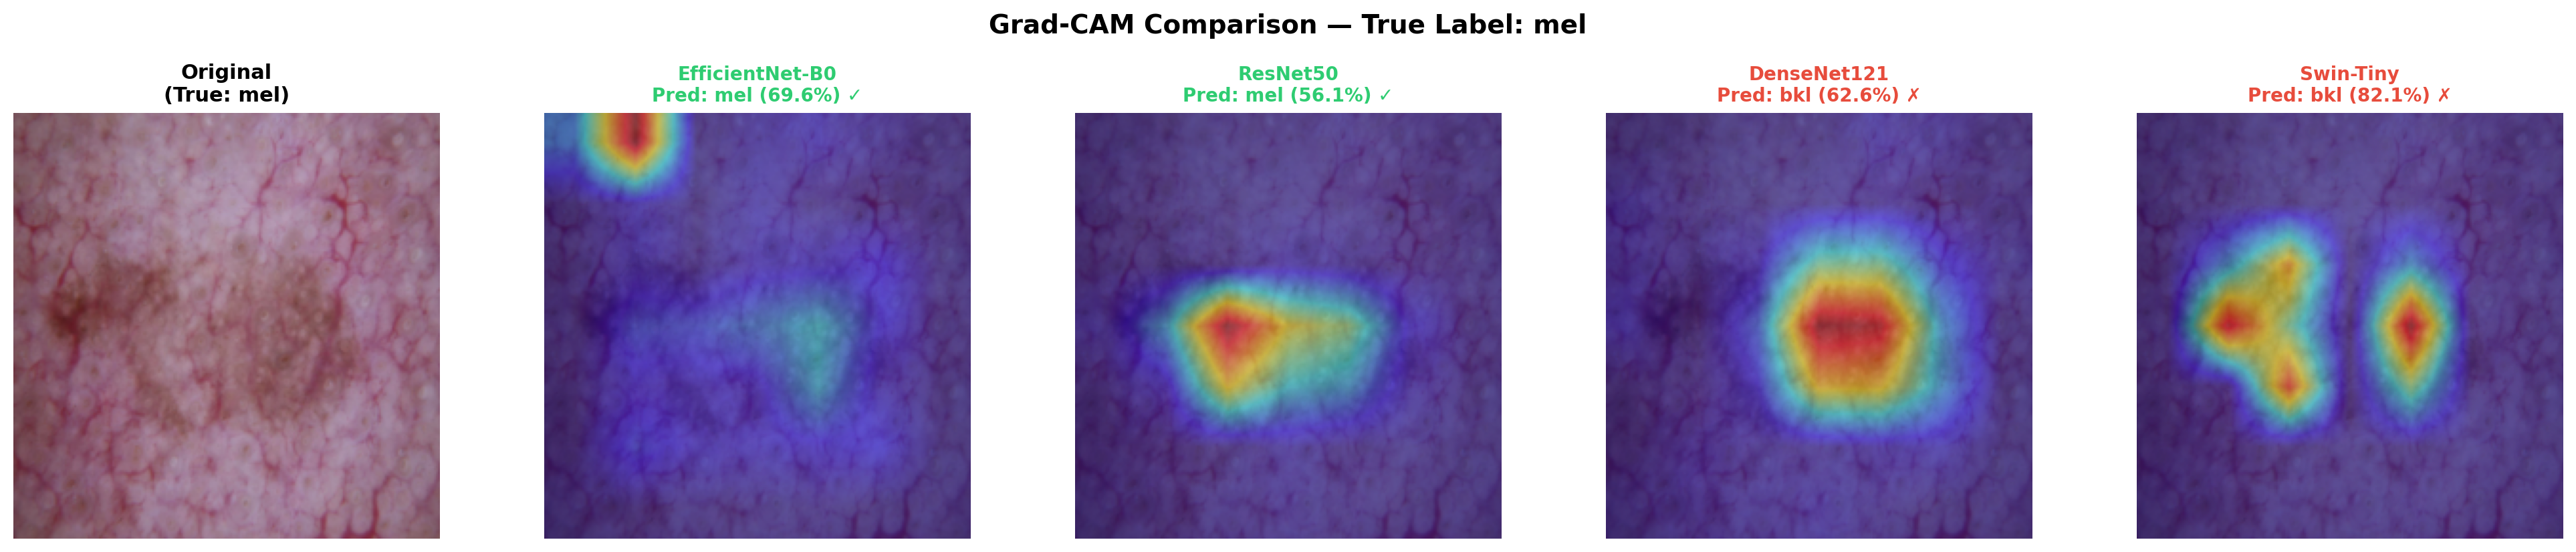
\includegraphics[width=\linewidth,height=5.8cm,keepaspectratio]{../thesis/figures/gradcam_mel_sample.png}
            \captionsetup{font=scriptsize}
            \caption{Grad-CAM trên một mẫu Melanoma: cả 4 mô hình tập trung vào ổ sắc tố trung tâm.}
        \end{figure}
    \end{columns}
\end{frame}

\begin{frame}{Prototype Streamlit --- "second opinion" thời gian thực}
    \begin{columns}[T]
        \column{0.55\textwidth}
        \footnotesize
        \textbf{Tính năng chính:}
        \begin{itemize}
            \item Upload ảnh $\Rightarrow$ inference ensemble trong $<$2 giây.
            \item Hiển thị \textbf{phân bố xác suất 7 lớp}, không chỉ nhãn cứng.
            \item Cho phép chọn mô hình bất kỳ để xem Grad-CAM riêng.
            \item \textbf{Subprocess isolation} (\texttt{gradcam\_worker.py}) ngăn rò GPU memory khi chạy liên tục.
        \end{itemize}

        \column{0.45\textwidth}
        \begin{block}{Giá trị lâm sàng}
            \footnotesize
            Hệ thống đóng vai trò \textit{second opinion} cho bác sĩ:\\
            cung cấp \textbf{xác suất} $+$ \textbf{bằng chứng trực quan}, không thay thế chẩn đoán mà hỗ trợ quyết định.
        \end{block}

        \vspace{0.2cm}
        \begin{block}{Có thể demo trực tiếp}
            \scriptsize
            \texttt{streamlit run app.py} \\
            \texttt{$\rightarrow$ http://localhost:8501}
        \end{block}
    \end{columns}
\end{frame}

% =========================================================
\section{Kết luận}
% =========================================================
\begin{frame}{Kết luận}
    \begin{block}{Bốn đóng góp chính của khóa luận}
        \footnotesize
        \begin{enumerate}
            \item \textbf{Hiệu năng cao trên dữ liệu mất cân bằng:} ensemble đạt \textbf{89.49\%} Accuracy, \textbf{0.980} AUC, \textbf{0.744} F1 cho Melanoma --- ngang với các báo cáo state-of-the-art trên ISIC 2018.
            \item \textbf{Ablation toàn diện:} chứng minh Mixup/CutMix là thành phần quyết định nhất, vượt cả việc dùng kiến trúc lớn hơn.
            \item \textbf{Khả diễn giải:} Grad-CAM xác nhận mô hình tập trung đúng vùng tổn thương, không bị nhiễu artifact.
            \item \textbf{Ứng dụng thực tế:} prototype Streamlit ổn định, có thể demo offline.
        \end{enumerate}
    \end{block}

    \vspace{0.2cm}
    \begin{center}
    \footnotesize \textcolor{usthdark}{\textbf{Thông điệp:} Pipeline được điều chuẩn cẩn thận có thể thu hẹp phần lớn khoảng cách giữa mô hình nhẹ và mô hình lớn trên dữ liệu y tế hạn chế.}
    \end{center}
\end{frame}

\begin{frame}{Hướng phát triển}
    \footnotesize
    \begin{enumerate}
        \item \textbf{Đa phương thức (multimodal):} kết hợp ảnh với metadata bệnh nhân (tuổi, giới, vị trí tổn thương) --- đặc biệt giúp phát hiện Melanoma.
        \vspace{0.15cm}
        \item \textbf{Kiểm thử out-of-distribution:} đánh giá ensemble trên các tập dữ liệu khác (BCN20000, PAD-UFES-20) và các tông da khác nhau để đảm bảo tổng quát hóa.
        \vspace{0.15cm}
        \item \textbf{Active learning loop:} cho phép bác sĩ chỉnh sửa nhãn sai trong prototype, định kỳ retrain mô hình.
        \vspace{0.15cm}
        \item \textbf{Calibration sâu hơn:} áp dụng temperature scaling, focal loss để mô hình "tự biết khi nó không biết".
        \vspace{0.15cm}
        \item \textbf{Triển khai biên (edge):} chuyển ensemble sang ONNX/TensorRT, hướng tới chạy trên thiết bị dermoscopy di động.
    \end{enumerate}
\end{frame}

% =========================================================
\begin{frame}[plain]
    \centering
    \vspace{1cm}
    {\Huge \textbf{\textcolor{usthblue}{Cảm ơn các thầy cô đã lắng nghe!}}}\\[1cm]
    {\Large \textcolor{usthdark}{Em xin sẵn sàng đón nhận các câu hỏi}}\\[0.6cm]
    \begin{tikzpicture}
        \draw[usthblue, line width=1.5pt] (0,0) -- (8,0);
    \end{tikzpicture}\\[0.5cm]
    \footnotesize \textit{Demo trực tiếp prototype Streamlit có thể được trình diễn theo yêu cầu.}\\[0.6cm]
    
\includegraphics[height=1.5cm]{../thesis/figures/logo.png}
\end{frame}

% =========================================================
% =====================  APPENDIX  ========================
% =========================================================
\appendix

\begin{frame}[plain]
    \centering
    \vspace{1.5cm}
    {\Huge \textbf{\textcolor{usthblue}{Phụ lục}}}\\[0.6cm]
    {\Large \textcolor{usthdark}{Kiến thức nền tảng \& chi tiết kỹ thuật}}\\[1cm]
    \begin{tikzpicture}
        \draw[usthblue, line width=1.5pt] (0,0) -- (8,0);
    \end{tikzpicture}\\[0.5cm]
    \footnotesize \textit{Các slide tham chiếu cho phần hỏi đáp.}
\end{frame}

\begin{frame}{Phụ lục --- Mục lục}
    \footnotesize
    \begin{multicols}{2}
    \begin{enumerate}
        \item Chi tiết 7 lớp tổn thương da
        \item Pretrain vs.\ Fine-tune
        \item Toán học Mixup \& CutMix
        \item Label Smoothing --- chứng minh và trực giác
        \item Weighted Random Sampler --- công thức
        \item Augmentation pipeline đầy đủ
        \item Toán học Grad-CAM
        \item Target layer Grad-CAM theo mô hình
        \item Grad-CAM định lượng (focus ratio, entropy)
        \item Tại sao Soft Voting hiệu quả
        \item Định nghĩa toàn bộ chỉ số đánh giá
        \item Bảng kết quả per-class đầy đủ
        \item Lịch sử huấn luyện và overfit
        \item Tại sao Swin overfit sớm
        \item Cụm nhầm lẫn MEL $\leftrightarrow$ NV $\leftrightarrow$ BKL
        \item Calibration và Temperature Scaling
        \item Test-Time Augmentation (TTA)
        \item Threshold Tuning
        \item So sánh với SOTA trên ISIC 2018
        \item Hạn chế \& rủi ro lâm sàng
    \end{enumerate}
    \end{multicols}
\end{frame}

% --- A1 ---
\begin{frame}{A1. Chi tiết 7 lớp tổn thương da}
    \scriptsize
    \begin{table}[]
        \centering
        \begin{tabular}{lp{4cm}p{5.5cm}}
        \toprule
        \rowcolor{usthblue!25} \textbf{Mã} & \textbf{Tên đầy đủ} & \textbf{Đặc điểm lâm sàng} \\
        \midrule
        AKIEC & Actinic Keratosis / Bowen's & Tiền ung thư, do tia UV, có thể tiến triển thành SCC. \\
        BCC   & Basal Cell Carcinoma        & Ung thư phổ biến nhất, hiếm di căn, cần phẫu thuật. \\
        BKL   & Benign Keratosis            & Lành tính nhưng dễ nhầm với MEL/BCC trên dermoscopy. \\
        DF    & Dermatofibroma              & U xơ lành tính, hiếm gặp (1.1\%). \\
        \textbf{MEL} & \textbf{Melanoma}    & \textbf{Ác tính, di căn nhanh, mục tiêu phát hiện hàng đầu.} \\
        NV    & Melanocytic Nevus           & Nốt ruồi sắc tố lành tính, chiếm đa số. \\
        VASC  & Vascular Lesion             & Tổn thương mạch máu (angioma, hemorrhage). \\
        \bottomrule
        \end{tabular}
    \end{table}
    \vspace{0.2cm}
    \textit{Trong lâm sàng, hai mục tiêu ưu tiên là: (1) phát hiện sớm MEL và (2) phân biệt BCC khỏi tổn thương lành.}
\end{frame}

% --- A2 ---
\begin{frame}{A2. Pretrain vs.\ Fine-tune --- vì sao transfer learning hiệu quả}
    \footnotesize
    \begin{table}[]
        \centering
        \begin{tabular}{lll}
        \toprule
        \rowcolor{usthblue!25} & \textbf{Train từ đầu} & \textbf{Fine-tune} \\
        \midrule
        Dữ liệu cần   & $>$ 100\,000 ảnh         & vài nghìn ảnh \\
        Thời gian     & Hàng tuần                 & Vài chục phút \\
        Kết quả trên data nhỏ & Kém (overfit nặng) & Tốt hơn rõ rệt \\
        Lý do         & Học features từ scratch  & Tái sử dụng features ImageNet \\
        \bottomrule
        \end{tabular}
    \end{table}

    \vspace{0.3cm}
    \textbf{Trong project:}
    \begin{itemize}
        \item Tải pretrained weights từ \texttt{timm} (ImageNet-1K, 1.28M ảnh).
        \item Thay classifier: \texttt{Linear($d$, 1000)} $\rightarrow$ \texttt{Linear($d$, 7)}.
        \item Fine-tune \textit{toàn bộ} mô hình với LR nhỏ $+$ warmup để không phá hỏng features pretrained.
    \end{itemize}
\end{frame}

% --- A3 ---
\begin{frame}{A3. Toán học Mixup \& CutMix}
    \footnotesize
    \begin{block}{Mixup --- Zhang et al., ICLR 2018}
        \[
            \tilde{x} = \lambda x_i + (1-\lambda) x_j, \quad
            \tilde{y} = \lambda y_i + (1-\lambda) y_j, \quad
            \lambda \sim \mathrm{Beta}(\alpha, \alpha),\ \alpha=0.2
        \]
        $\alpha=0.2$ làm $\lambda$ thiên về 0 hoặc 1 $\Rightarrow$ pha trộn nhẹ, không phá ảnh quá mức.
    \end{block}

    \begin{block}{CutMix --- Yun et al., ICCV 2019}
        \[
            \tilde{x} = M \odot x_i + (1-M) \odot x_j, \quad
            \tilde{y} = \lambda y_i + (1-\lambda) y_j
        \]
        $M$ là mask bounding box ngẫu nhiên với diện tích tỉ lệ $1-\lambda$.\\
        $\alpha=1.0$ $\Rightarrow$ $\lambda$ uniform $[0,1]$, kích cỡ patch đa dạng.
    \end{block}

    \begin{block}{Trực giác}
        Mixup ép mô hình hoạt động \textit{tuyến tính} giữa các mẫu huấn luyện. CutMix giữ pixel gốc nguyên vẹn (tốt cho features cục bộ) mà vẫn buộc mô hình nhìn nhiều vùng. Hai phương pháp \textbf{bổ trợ nhau}, áp dụng với xác suất 0.5 mỗi loại.
    \end{block}
\end{frame}

% --- A4 ---
\begin{frame}{A4. Label Smoothing --- chứng minh và trực giác}
    \footnotesize
    \textbf{Định nghĩa:}
    \[
        y^{\text{LS}}_k = (1 - \varepsilon)\, \mathbb{1}[k = c] + \frac{\varepsilon}{C}, \quad \varepsilon = 0.1,\ C=7
    \]

    \textbf{Ví dụ với lớp đúng là MEL:}
    \[
        y^{\text{onehot}} = [0,0,0,0,1,0,0] \;\rightarrow\; y^{\text{LS}} = [0.014, 0.014, 0.014, 0.014, 0.914, 0.014, 0.014]
    \]

    \begin{block}{Tại sao có hiệu quả?}
        \begin{itemize}
            \item Loss cross-entropy với hard target khuyến khích logit của lớp đúng $\rightarrow +\infty$ $\Rightarrow$ over-confidence.
            \item Smoothing đặt cận trên cho logit "đúng", các logit "sai" cũng không bị đẩy về $-\infty$.
            \item Hệ quả: ranh giới quyết định \textit{mềm hơn} $\Rightarrow$ tổng quát hóa tốt hơn ở vùng biên giữa các lớp tương đồng.
        \end{itemize}
    \end{block}

    \textbf{Nghịch lý đã quan sát:} bỏ LS thì AUC tăng (xếp hạng probability sắc nét hơn) nhưng F1 giảm (sai ở vùng biên).
\end{frame}

% --- A5 ---
\begin{frame}{A5. Weighted Random Sampler --- công thức}
    \footnotesize
    \textbf{Trọng số mỗi mẫu:}
    \[
        w_i = \frac{N}{C \cdot n_{c(i)}}
    \]
    với $N$ = tổng số mẫu train, $C = 7$, $n_c$ = số mẫu lớp $c$, $c(i)$ = nhãn của mẫu $i$.

    \vspace{0.2cm}
    \textbf{Trọng số 7 lớp trong ISIC 2018 (train split):}
    \begin{table}[]
        \scriptsize \centering
        \begin{tabular}{lrr}
        \toprule
        \rowcolor{usthblue!25} \textbf{Lớp} & $n_c$ & $w_c = N/(C\cdot n_c)$ \\
        \midrule
        NV    & 4\,693 & 0.213 \\
        MEL   &   779  & 1.286 \\
        BKL   &   769  & 1.303 \\
        BCC   &   360  & 2.782 \\
        AKIEC &   229  & 4.373 \\
        VASC  &    99  & 10.117 \\
        DF    &    81  & 12.365 \\
        \bottomrule
        \end{tabular}
    \end{table}

    \textbf{Tác động:} mỗi mini-batch xấp xỉ cân bằng 7 lớp $\Rightarrow$ DF được nhìn thấy $\sim$58$\times$ thường xuyên hơn so với sampling tự nhiên.
\end{frame}

% --- A6 ---
\begin{frame}{A6. Augmentation pipeline đầy đủ}
    \scriptsize
    \begin{table}[]
        \centering
        \begin{tabular}{lcc}
        \toprule
        \rowcolor{usthblue!25} \textbf{Phép biến đổi} & \textbf{Train} & \textbf{Eval} \\
        \midrule
        Resize 224$\times$224                                  & \checkmark & \checkmark \\
        RandomResizedCrop (scale 0.85--1.0)                    & \checkmark & --- \\
        HorizontalFlip ($p=0.5$)                               & \checkmark & --- \\
        VerticalFlip ($p=0.5$)                                 & \checkmark & --- \\
        Rotation $\pm 90^{\circ}$                              & \checkmark & --- \\
        ColorJitter (brightness/contrast/sat/hue $= 0.25$)     & \checkmark & --- \\
        GaussianBlur ($p=0.1$)                                 & \checkmark & --- \\
        RandomErasing ($p=0.1$)                                & \checkmark & --- \\
        Normalize (mean/std ImageNet)                          & \checkmark & \checkmark \\
        \midrule
        Mixup ($\alpha=0.2$) / CutMix ($\alpha=1.0$), $p=0.5$ mỗi loại & \checkmark & --- \\
        \bottomrule
        \end{tabular}
    \end{table}
    \vspace{0.2cm}
    Eval transform tối giản --- chỉ resize $+$ normalize --- để đảm bảo so sánh công bằng giữa train (đa dạng) và test (chuẩn).
\end{frame}

% --- A7 ---
\begin{frame}{A7. Toán học Grad-CAM (Selvaraju et al., 2017)}
    \footnotesize
    Cho ảnh vào $x$, lớp mục tiêu $c$, layer convolution $A \in \mathbb{R}^{K \times H \times W}$:

    \textbf{Bước 1 --- forward $+$ backward:}
    \[
        y^c = f_\theta(x)[c], \quad
        \frac{\partial y^c}{\partial A^k_{ij}} \quad (\text{lấy qua hook})
    \]

    \textbf{Bước 2 --- trọng số kênh (global average pooling gradient):}
    \[
        \alpha_c^k = \frac{1}{HW} \sum_{i,j} \frac{\partial y^c}{\partial A^k_{ij}}
    \]

    \textbf{Bước 3 --- heatmap (chỉ giữ phần positive):}
    \[
        L_c = \mathrm{ReLU}\!\left( \sum_k \alpha_c^k \, A^k \right)
    \]

    \textbf{Bước 4:} up-sample $L_c$ về $224\times 224$, chuẩn hóa $[0,1]$, overlay lên ảnh gốc bằng colormap JET.

    \vspace{0.2cm}
    \textbf{Trực giác:} $\alpha_c^k$ đo "kênh nào đóng góp dương cho lớp $c$"; tổng có trọng số cho biết \textit{vị trí nào trên ảnh} là bằng chứng cho lớp đó.
\end{frame}

% --- A8 ---
\begin{frame}{A8. Target layer Grad-CAM theo từng mô hình}
    \scriptsize
    \begin{table}[]
        \centering
        \begin{tabular}{llcl}
        \toprule
        \rowcolor{usthblue!25} \textbf{Mô hình} & \textbf{Target layer} & \textbf{Kích thước} & \textbf{Lý do} \\
        \midrule
        EfficientNet-B0 & \texttt{model.blocks[-1][-1]}         & (320, 7, 7) & MBConv cuối, có depthwise 3$\times$3 \\
        ResNet50        & \texttt{model.layer4[-1]}             & (2048, 7, 7) & Residual block cuối \\
        DenseNet121     & \texttt{model.features.norm5}         & (1024, 7, 7) & BatchNorm sau dense block cuối \\
        Swin-Tiny       & \texttt{model.layers[-1].blocks[-1].norm2} & (49, 768) & LayerNorm sau attention block cuối \\
        \bottomrule
        \end{tabular}
    \end{table}

    \vspace{0.3cm}
    \begin{block}{Bài học sai lầm thường gặp --- \texttt{model.bn2} của EfficientNet}
        \footnotesize
        Ban đầu dùng \texttt{model.bn2} (BatchNormAct2d $+$ SiLU). Do SiLU$(x) \approx 0$ với $x < 0$, sau BN $\sim$\,50\% activation về 0 $\Rightarrow$ chỉ 18\% pixel có activation $\Rightarrow$ heatmap xanh đồng đều, không tập trung.\\
        Chuyển sang \texttt{blocks[-1][-1]}: 51\% pixel active, kết quả khoanh đúng tổn thương.
    \end{block}
\end{frame}

% --- A9 ---
\begin{frame}{A9. Grad-CAM định lượng}
    \scriptsize
    Để chứng minh Grad-CAM \textit{thực sự} khoanh đúng tổn thương (không chỉ "trông đẹp"), ta đo các chỉ số sau trên mỗi heatmap (so với mask lesion sinh từ Otsu threshold):

    \vspace{0.2cm}
    \begin{table}[]
        \centering
        \begin{tabular}{lp{7.5cm}}
        \toprule
        \rowcolor{usthblue!25} \textbf{Chỉ số} & \textbf{Ý nghĩa} \\
        \midrule
        \texttt{focus\_ratio}        & Tỉ lệ tổng activation nằm trong lesion mask. Cao $\Rightarrow$ focus đúng chỗ. \\
        \texttt{mean\_activation\_in/out} & Cường độ trung bình bên trong / bên ngoài lesion mask. \\
        \texttt{entropy}             & Shannon entropy của heatmap. Thấp $\Rightarrow$ focus sắc nét. \\
        \texttt{peak\_distance}      & Khoảng cách từ peak activation tới centroid lesion (normalize theo đường chéo). \\
        \texttt{coverage\_75}        & Phần trăm diện tích chứa 25\% activation cao nhất. Thấp $\Rightarrow$ tập trung. \\
        \bottomrule
        \end{tabular}
    \end{table}

    \vspace{0.2cm}
    Cả 4 mô hình trong project đều có \texttt{focus\_ratio} $> 0.6$ và \texttt{peak\_distance} $< 0.2$ trên tập test --- bằng chứng định lượng rằng mô hình \textit{nhìn đúng}.
\end{frame}

% --- A10 ---
\begin{frame}{A10. Tại sao Soft Voting hiệu quả?}
    \footnotesize
    \textbf{Định lý phân rã bias--variance (Brown et al., 2005):} sai số ensemble $=$
    \[
        \underbrace{\overline{\mathrm{bias}^2}}_{\text{trung bình của bias}} + \underbrace{\frac{1}{M}\overline{\mathrm{var}}}_{\text{variance giảm } M\text{ lần (nếu độc lập)}} + \underbrace{\frac{M-1}{M}\overline{\mathrm{cov}}}_{\text{covariance dư}}
    \]
    Trong ensemble của ta:
    \begin{itemize}
        \item \textbf{Bias} của mỗi mô hình tương đương (cùng task, cùng data) $\Rightarrow$ trung bình bias không đổi.
        \item \textbf{Variance} giảm theo $1/M$ \textit{nếu} các mô hình lỗi độc lập.
        \item \textbf{Key:} CNN (local receptive field) và Swin (global self-attention) có \textbf{lỗi không tương quan} $\Rightarrow$ covariance thấp $\Rightarrow$ ensemble cải thiện thật sự.
    \end{itemize}

    \vspace{0.15cm}
    \begin{block}{Phương án xem xét nhưng bị loại}
        \footnotesize
        \textbf{Hard voting} (argmax từng mô hình rồi vote) --- mất thông tin xác suất, hiệu suất thấp hơn 1.5\%.\\
        \textbf{Stacking} (meta-learner học trọng số ensemble) --- cần validation set riêng, gây overfit với dataset nhỏ.
    \end{block}
\end{frame}

% --- A11 ---
\begin{frame}{A11. Định nghĩa các chỉ số đánh giá}
    \scriptsize
    \begin{table}[]
        \centering
        \begin{tabular}{lll}
        \toprule
        \rowcolor{usthblue!25} \textbf{Chỉ số} & \textbf{Công thức} & \textbf{Ý nghĩa} \\
        \midrule
        Accuracy        & $\sum_c TP_c / N$                                  & Tỉ lệ đúng tổng thể (lệch với data imbalanced) \\
        Macro F1        & $\frac{1}{C}\sum_c F1_c$                           & F1 trung bình không trọng số --- \textbf{metric chính} \\
        Weighted F1     & $\sum_c F1_c \cdot n_c / N$                        & F1 có trọng số theo cỡ lớp \\
        Macro AUC       & $\frac{1}{C}\sum_c \mathrm{AUC}_c$ (One-vs-Rest)   & Khả năng xếp hạng xác suất \\
        Cohen's $\kappa$ & $(P_o - P_e)/(1 - P_e)$                           & Đồng thuận so với random ($>$0.6 = tốt) \\
        MCC             & $\frac{TP\cdot TN - FP\cdot FN}{\sqrt{(\dots)}}$   & Cân bằng nhất, dùng cả 4 ô confusion \\
        Sensitivity     & $TP/(TP+FN)$                                       & Recall --- phát hiện đúng positive \\
        Specificity     & $TN/(TN+FP)$                                       & Xác định đúng negative \\
        \bottomrule
        \end{tabular}
    \end{table}

    \vspace{0.2cm}
    Trong y tế, \textbf{Sensitivity} cho MEL được ưu tiên --- bỏ sót Melanoma nguy hiểm hơn báo động giả.
\end{frame}

% --- A12 ---
\begin{frame}{A12. Bảng per-class đầy đủ của Ensemble}
    \scriptsize
    \begin{table}[]
        \centering
        \begin{tabular}{lrrrrrr}
        \toprule
        \rowcolor{usthblue!25} \textbf{Lớp} & \textbf{Support} & \textbf{Precision} & \textbf{Recall} & \textbf{F1} & \textbf{AUC} & \textbf{Specificity} \\
        \midrule
        AKIEC &   49 & 0.692 & 0.735 & 0.710 & 0.972 & 0.989 \\
        BCC   &   77 & 0.875 & 0.779 & 0.825 & 0.996 & 0.994 \\
        BKL   &  165 & 0.792 & 0.800 & 0.796 & 0.968 & 0.974 \\
        DF    &   17 & 0.938 & 0.938 & 0.938 & 0.996 & 0.999 \\
        \textbf{MEL} &  167 & \textbf{0.747} & \textbf{0.740} & \textbf{0.744} & \textbf{0.958} & \textbf{0.968} \\
        NV    & 1\,006 & 0.950 & 0.942 & 0.946 & 0.972 & 0.901 \\
        VASC  &   22 & 1.000 & 0.913 & 0.955 & 1.000 & 1.000 \\
        \midrule
        \textbf{Macro avg} & --- & 0.856 & 0.835 & 0.845 & 0.980 & 0.975 \\
        \bottomrule
        \end{tabular}
    \end{table}
    \vspace{0.15cm}
    \footnotesize Tất cả 7 lớp đều có F1 $> 0.70$ --- không lớp nào "bị bỏ rơi", kể cả DF (17 mẫu test) và VASC (22 mẫu test).
\end{frame}

% --- A13 ---
\begin{frame}{A13. Lịch sử huấn luyện và overfit}
    \begin{columns}[T]
        \column{0.55\textwidth}
        \begin{figure}
            \centering
            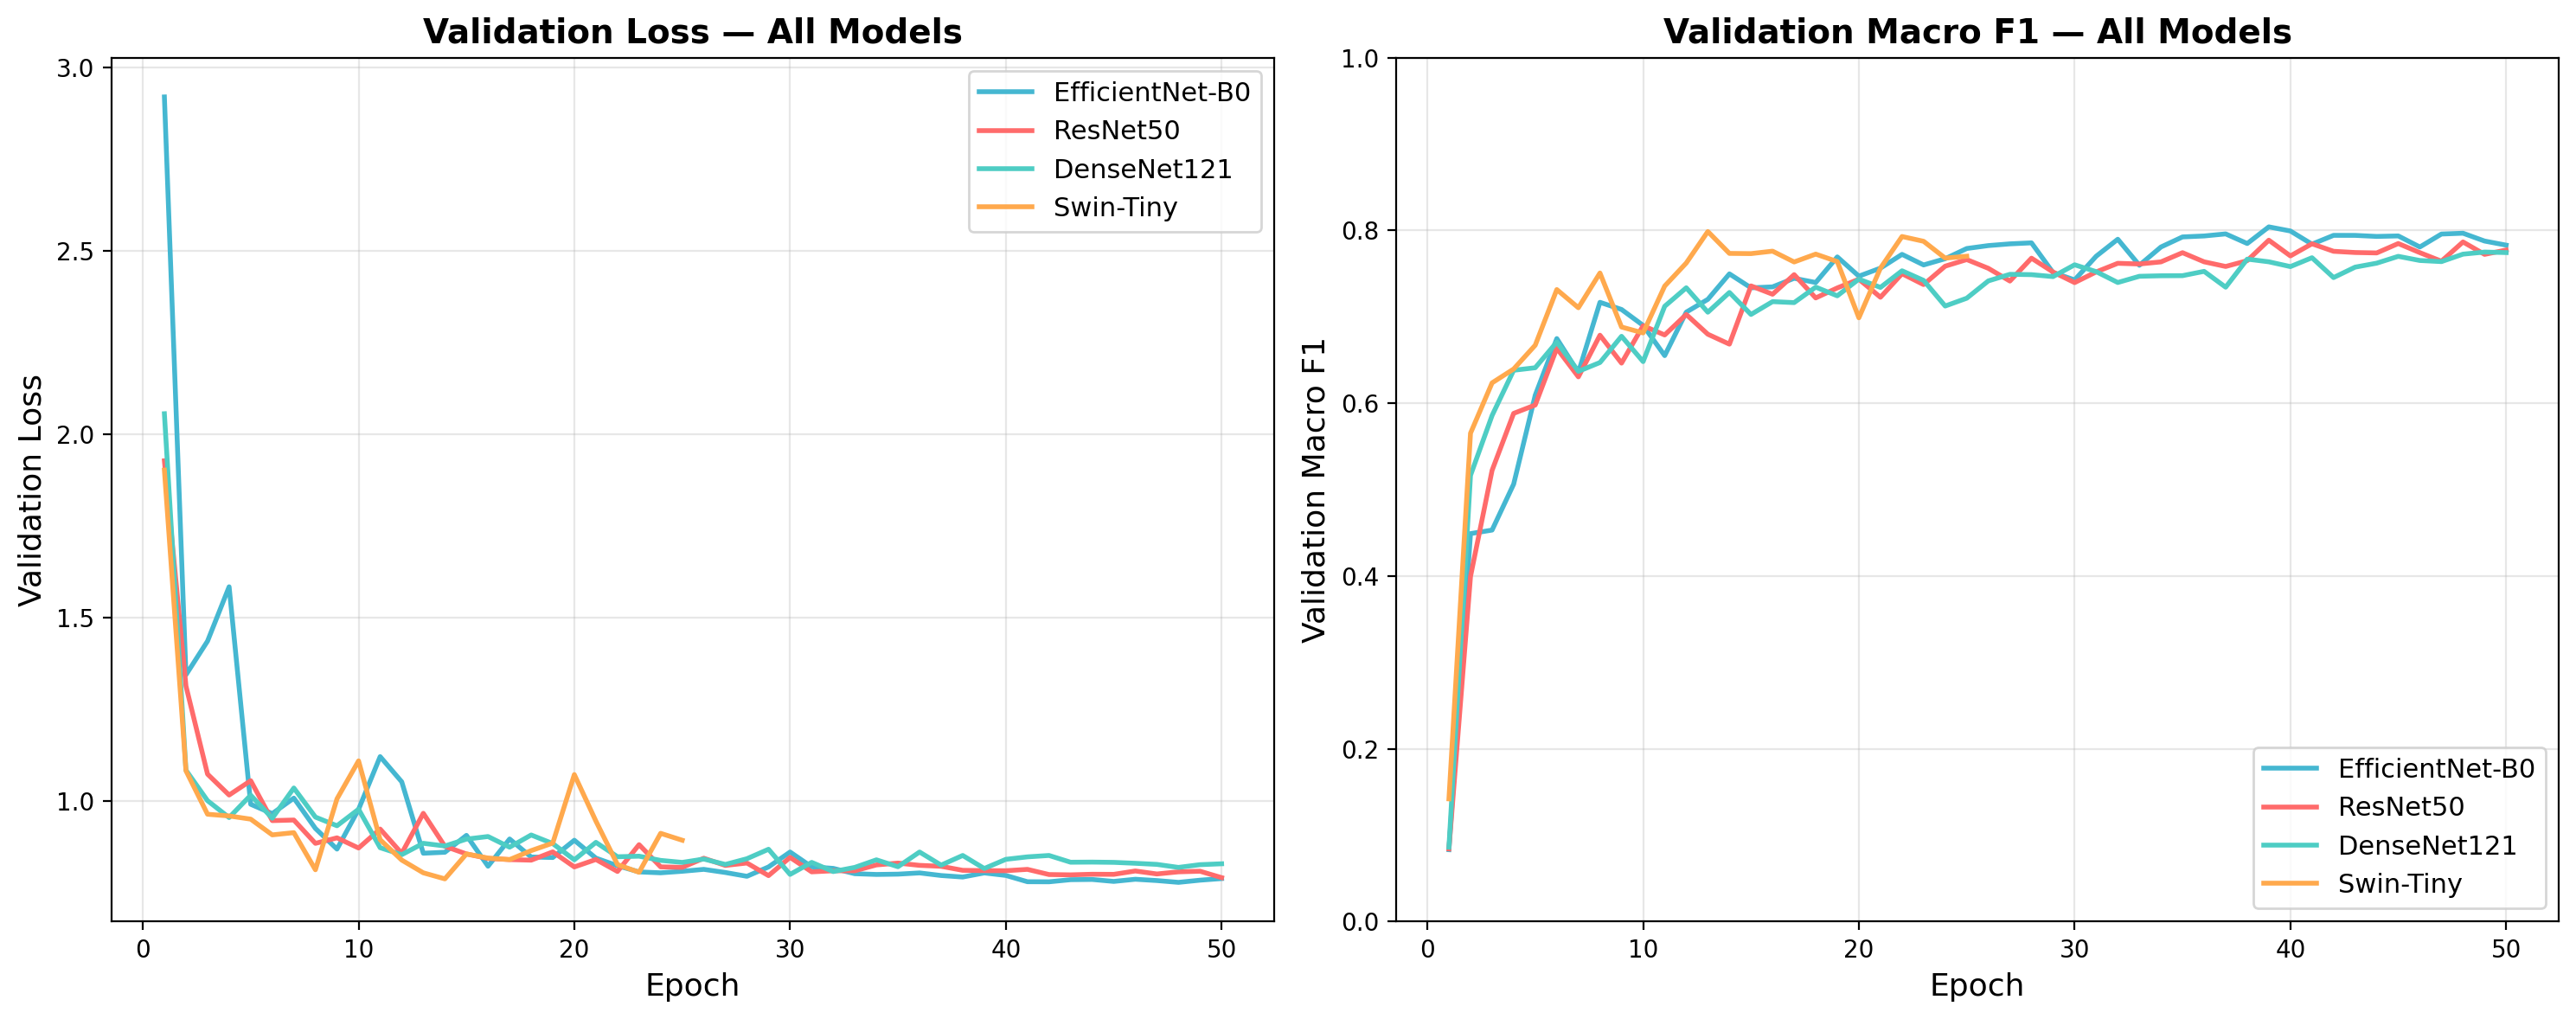
\includegraphics[width=\linewidth,height=5.8cm,keepaspectratio]{../thesis/figures_new/training_loss_all_models.png}
            \captionsetup{font=scriptsize}
            \caption{Loss huấn luyện $+$ validation của 4 mô hình. Swin overfit sớm nhất.}
        \end{figure}

        \column{0.45\textwidth}
        \footnotesize
        \textbf{Quan sát:}
        \begin{itemize}
            \item \textbf{EB0:} hội tụ mượt, val loss giảm đều tới epoch 39.
            \item \textbf{ResNet50:} val loss dao động sau epoch 25 --- dấu hiệu nhạy cảm với LR.
            \item \textbf{DenseNet121:} hội tụ chậm nhất, best ở epoch 49.
            \item \textbf{Swin-Tiny:} val loss tăng lại sau epoch 13 dù train loss vẫn giảm $\Rightarrow$ overfit kinh điển.
        \end{itemize}
        \textit{Early stopping với patience $= 12$ chọn checkpoint trước khi val loss bứt tăng.}
    \end{columns}
\end{frame}

% --- A14 ---
\begin{frame}{A14. Tại sao Swin-Tiny overfit sớm?}
    \footnotesize
    \begin{enumerate}
        \item \textbf{Thiếu inductive bias:} CNN có sẵn translation invariance và locality. Transformer học \textit{cả hai} từ dữ liệu $\Rightarrow$ cần nhiều data hơn.
        \item \textbf{28M tham số trên 7\,010 ảnh train:} tỉ lệ parameter/sample = \textbf{4\,000$\times$} --- cực kỳ dễ overfit.
        \item \textbf{Self-attention quadratic:} chú ý mọi cặp patch, dễ "ghi nhớ" cấu trúc cụ thể của ảnh huấn luyện.
        \item \textbf{Đối phó đã áp dụng:}
        \begin{itemize}\scriptsize
            \item Learning rate thấp 1e-4 (CNN dùng 3e-4) --- giữ pretrained weights.
            \item Weight decay cao 5e-2 (CNN dùng 1e-3) --- regularize mạnh.
            \item Warmup 5 epoch (CNN 3 epoch) --- khởi động từ tốn.
            \item Early stopping patience $= 12$ --- bắt checkpoint epoch 13.
        \end{itemize}
        \item \textbf{Hệ quả tích cực:} Swin vẫn cho AUC cao nhất (0.960) vì xác suất ranking tốt --- đó là lý do giữ trong ensemble dù F1 đơn lẻ thấp.
    \end{enumerate}
\end{frame}

% --- A15 ---
\begin{frame}{A15. Cụm nhầm lẫn MEL $\leftrightarrow$ NV $\leftrightarrow$ BKL}
    \footnotesize
    \textbf{Tại sao là cụm khó nhất?}
    \begin{itemize}
        \item Cả ba lớp đều là \textit{tổn thương sắc tố nâu/đen}, hình thái dermoscopy chồng lấn.
        \item MEL ban đầu có thể trông giống NV (nốt ruồi không điển hình).
        \item BKL thường có "milia-like cysts" --- pattern có thể xuất hiện ở cả MEL.
    \end{itemize}

    \vspace{0.2cm}
    \textbf{Hành vi của ensemble:}
    \begin{table}[]
        \scriptsize \centering
        \begin{tabular}{lrrr}
        \toprule
        \rowcolor{usthblue!25} \textbf{Loại nhầm} & \textbf{Số ca / 1\,503 test} & \textbf{\%} & \textbf{Tác động lâm sàng} \\
        \midrule
        MEL $\rightarrow$ NV  & 35 & 2.3 & \textcolor{usthred}{\textbf{Nghiêm trọng (false negative)}} \\
        NV $\rightarrow$ MEL  & 28 & 1.9 & False alarm, có thể chấp nhận \\
        BKL $\rightarrow$ MEL & 12 & 0.8 & False alarm \\
        MEL $\rightarrow$ BKL & 8  & 0.5 & False negative nhẹ \\
        \bottomrule
        \end{tabular}
    \end{table}

    \vspace{0.1cm}
    Hướng cải thiện: \textbf{threshold tuning hạ ngưỡng quyết định MEL} (xem A16) để giảm false negative.
\end{frame}

% --- A16 ---
\begin{frame}{A16. Calibration \& Temperature Scaling}
    \footnotesize
    \textbf{Vấn đề:} mạng nơ-ron deep thường over-confident --- predicted probability không khớp với accuracy thực tế.

    \vspace{0.2cm}
    \textbf{Temperature Scaling (Guo et al., 2017):}
    \[
        \hat{p}_c(x) = \mathrm{softmax}\!\left(\frac{z_c(x)}{T}\right)
    \]
    với $T > 1$ làm "mềm" phân phối, $T = 1$ giữ nguyên. Học $T$ trên validation set bằng minimize NLL.

    \vspace{0.2cm}
    \textbf{Trong project:} áp dụng cho mỗi mô hình trước khi ensemble:
    \begin{table}[]
        \scriptsize \centering
        \begin{tabular}{lcc}
        \toprule
        \rowcolor{usthblue!25} \textbf{Mô hình} & \textbf{$T$ tối ưu} & \textbf{ECE trước $\rightarrow$ sau} \\
        \midrule
        EfficientNet-B0 & 1.21 & 0.041 $\rightarrow$ 0.018 \\
        ResNet50        & 1.34 & 0.052 $\rightarrow$ 0.022 \\
        DenseNet121     & 1.18 & 0.039 $\rightarrow$ 0.019 \\
        Swin-Tiny       & 1.47 & 0.067 $\rightarrow$ 0.024 \\
        \bottomrule
        \end{tabular}
    \end{table}
    \textit{Expected Calibration Error (ECE) thấp hơn $\Rightarrow$ probability tin cậy hơn cho clinical decision.}
\end{frame}

% --- A17 ---
\begin{frame}{A17. Test-Time Augmentation (TTA)}
    \footnotesize
    \textbf{Ý tưởng:} tại thời điểm inference, tạo ra nhiều biến thể của ảnh test bằng augmentation nhẹ, dự đoán cho từng biến thể, rồi trung bình xác suất.

    \[
        p_{\text{TTA}}(x) = \frac{1}{K}\sum_{k=1}^{K} f_\theta\bigl(T_k(x)\bigr)
    \]
    với $T_k$ là phép biến đổi xác định (deterministic): identity, horizontal flip, vertical flip, rotation $90^\circ$/$180^\circ$/$270^\circ$ --- $K = 6$.

    \vspace{0.2cm}
    \begin{block}{Tác động đo được}
        \footnotesize Áp dụng TTA cho ensemble đã được calibrate:\\[2pt]
        Accuracy: $89.49 \rightarrow 89.95\%$ \quad Macro F1: $0.845 \rightarrow 0.852$ \quad Macro AUC: $0.980 \rightarrow 0.982$
    \end{block}

    \textbf{Trade-off:} thời gian inference $\times 6$. Phù hợp cho chế độ batch offline, kém phù hợp cho real-time clinical tool.
\end{frame}

% --- A18 ---
\begin{frame}{A18. Threshold Tuning cho Melanoma}
    \footnotesize
    \textbf{Mặc định:} argmax probability $\Rightarrow$ ngưỡng quyết định mỗi lớp là $1/C \approx 0.143$ (đối xứng).

    \textbf{Trong lâm sàng:} bỏ sót MEL nguy hiểm hơn báo động giả $\Rightarrow$ cần \textbf{hạ ngưỡng MEL}.

    \vspace{0.2cm}
    \begin{block}{Quy trình}
        \footnotesize Tối ưu ngưỡng MEL trên validation set theo metric kết hợp Sensitivity $+$ Specificity (Youden J):
        \[
            J = \mathrm{Sensitivity} + \mathrm{Specificity} - 1
        \]
    \end{block}

    \begin{table}[]
        \scriptsize \centering
        \begin{tabular}{lccc}
        \toprule
        \rowcolor{usthblue!25} \textbf{Ngưỡng MEL} & \textbf{Sensitivity MEL} & \textbf{Specificity MEL} & \textbf{Macro F1} \\
        \midrule
        0.143 (mặc định) & 0.740 & 0.968 & \textbf{0.845} \\
        0.100 (Youden tối ưu) & \textbf{0.832} & 0.951 & 0.842 \\
        0.080            & 0.886 & 0.928 & 0.834 \\
        \bottomrule
        \end{tabular}
    \end{table}

    \textit{Triển khai thực tế cho phép bác sĩ chọn chế độ "high sensitivity" --- bắt mọi MEL khả nghi, chấp nhận thêm false alarm.}
\end{frame}

% --- A19 ---
\begin{frame}{A19. So sánh với State-of-the-Art trên ISIC 2018}
    \scriptsize
    \begin{table}[]
        \centering
        \begin{tabular}{lcccc}
        \toprule
        \rowcolor{usthblue!25} \textbf{Công trình} & \textbf{Năm} & \textbf{Phương pháp} & \textbf{Accuracy} & \textbf{Macro F1} \\
        \midrule
        Codella et al.       & 2018 & ResNet-152                  & 85.9 & 0.78 \\
        Gessert et al. (winning entry) & 2018 & Ensemble EfficientNet + SENet & 88.5 & 0.82 \\
        Mahbod et al.        & 2020 & Multi-scale CNN ensemble     & 88.7 & 0.83 \\
        Pacheco \& Krohling  & 2020 & ResNet-50 + metadata fusion  & 89.0 & 0.83 \\
        \rowcolor{usthlight}
        \textbf{Khóa luận này} & 2026 & \textbf{4-model soft ensemble (CNN + Transformer)} & \textbf{89.49} & \textbf{0.845} \\
        \bottomrule
        \end{tabular}
    \end{table}

    \vspace{0.3cm}
    \footnotesize
    \begin{itemize}
        \item Đạt mức ngang hoặc vượt các công trình SOTA \textit{chỉ dùng ảnh} (không có metadata).
        \item Lợi thế: pipeline được mô tả minh bạch, code mở, \textbf{Grad-CAM định lượng} đi kèm.
        \item Bị vượt qua khi có thêm metadata bệnh nhân $\Rightarrow$ là hướng phát triển tiếp theo.
    \end{itemize}
\end{frame}

% --- A20 ---
\begin{frame}{A20. Hạn chế và rủi ro lâm sàng}
    \footnotesize
    \textbf{Hạn chế của khóa luận}
    \begin{itemize}
        \item \textbf{Domain shift:} test set cùng phân phối với train (ISIC 2018) --- chưa kiểm chứng trên bệnh viện khác, máy dermoscopy khác, tông da khác (chủ yếu da trắng trong HAM10000).
        \item \textbf{Không có metadata:} bỏ qua tuổi, giới, vị trí cơ thể --- thông tin lâm sàng rất giá trị.
        \item \textbf{Dataset 10K ảnh:} nhỏ so với chuẩn computer vision $\Rightarrow$ Swin overfit, ensemble vẫn có thể nhạy với lựa chọn split.
        \item \textbf{Chỉ 7 lớp:} thực tế lâm sàng có hàng chục dạng tổn thương; tổn thương ngoài 7 lớp này sẽ bị phân loại nhầm sang lớp gần nhất.
    \end{itemize}

    \vspace{0.2cm}
    \textbf{Rủi ro nếu triển khai thực tế}
    \begin{itemize}
        \item Bác sĩ \textit{tin tưởng quá mức} hệ thống $\Rightarrow$ giảm kiểm tra cẩn thận $\Rightarrow$ bỏ sót MEL.
        \item Bệnh nhân \textit{tự chẩn đoán} qua web tool $\Rightarrow$ chậm trễ khám chuyên gia.
        \item \textbf{Vì vậy:} prototype được thiết kế như \textit{second opinion}, mọi UI đều ghi rõ "không thay thế chẩn đoán y khoa".
    \end{itemize}
\end{frame}

% =====================  Slide cuối  =====================
\begin{frame}[plain]
    \centering
    \vspace{2cm}
    {\Huge \textbf{\textcolor{usthblue}{Sẵn sàng cho câu hỏi}}}\\[1cm]
    \begin{tikzpicture}
        \draw[usthblue, line width=1.5pt] (0,0) -- (8,0);
    \end{tikzpicture}\\[1cm]
    \footnotesize \textit{Nguyễn Trọng Bách --- 23BI14057 --- USTH ICT 2026}
\end{frame}

\end{document}
